% !TEX root = ../thesis.tex
% !TeX spellcheck = en_US

% visibility graphs contain shortest paths
% adding source/destination nodes to graph and connecting them allows determination of shortest path between arbitrary locations in the presence of obstacles in the plain
% Connecting visibility edges to roads enables more flexible and realistic routes
% A* routing still fast (speedup methods can be applied) but connecting locations is slowing routing down
This thesis presented a routing algorithm that combines graph-based with geometric routing and was therefore called \emph{hybrid routing algorithm}.
It uses road data as well as open spaces between obstacles to find shortest path.

The geometric routing component is based on visibility graphs, which is a graph that contains only edges between vertices that are visible to each other, i.e. only edges that so not intersect any obstacle from the input dataset.
Edges in visibility graphs are therefore shortest paths between their vertices, which is a useful property for finding general shortest paths between vertices.
Generating a routable visibility graph is one core task of the hybrid routing algorithm.

Merging the visibility graph with the existing road edges from the input dataset is the second core task of the hybrid routing algorithm.
The challenge in this task is the connecting between a road edge and intersecting visibility edges to allow a graph-based routing algorithm to switch between these two types of edges.

The graph-based routing component consists of the popular A* algorithm, but any graph-based routing algorithm, including ones using speedup techniques, could be used.
Because source and destination coordinates of a routing query do not necessarily correspond to vertices in the routing graph, these location must be added to the graph.
After adding vertices for the source and destination, these two new vertices need to be connected to the surrounding graph in order to be reachable by the graph-based routing algorithm.

\section{Future work}
\label{sec:future-work}

	Even though the presented algorithm works as intended, some problems are known and the potential for further enhancements exists.
	This sections discusses these problems including potential solutions, lists additional technical enhancements as well as additional functionalities that might be beneficial for routing.

	\subsection{Known problems}
		% Overall: Speed up visibility edge generation for initial import + routing
		Even though it might not be a severe problem, the graph generation and routing performance offers potential to be improved, either by an optimization of the current implementation or by implementing a different graph generation algorithm.
		
		The first approach might use better data structured for vertices and obstacles.
		In the current implementation, for every vertex, ever other vertex in the dataset is considered a potential neighbor and then filtered out using e.g. valid angle and shadow areas.
		Using a QuadTree might increase performance for this process since not all vertices need to be checked.
		However, any additional data structure also introduces additional overhead and might only be beneficial for datasets of a certain size.
		The usefulness of this approach needs testing and evaluation.
		
		The second approach to reduce graph generation times is a complete reimplementation of the edge creation.
		Such a reimplementation might use approaches mentioned in \Cref{subsec:suitablilty-edge-creation-approaches}, which showed promising sub-quadratic runtime complexities.
		
		\begin{wrapfigure}{r}{0.35\textwidth}
			\vspace{-1.5\baselineskip}
			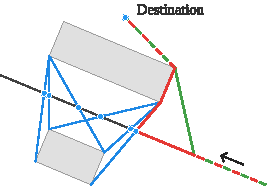
\includegraphics[width=\linewidth]{images/qgis-future-work-connectivity-problem}
			\caption{Connectivity problem in case of too few visibility edges. The green path might be the expected result but the red path is the actual shortest path.}
			\label{fig:connectivity-problem}
			\vspace{\baselineskip}
			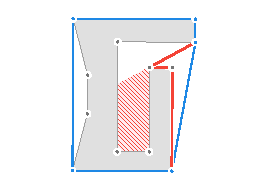
\includegraphics[width=\linewidth]{images/qgis-future-work-convex-hull-problem}
			\caption{Concave polygons do not always contain all necessary edges (red) but only those edges connecting the convex hull (blue). Some regions are therefore unreachable (red marked area).}
			\label{fig:convex-hull-problem}
		\end{wrapfigure}
				
		% Connection to roads based on the hope that there are many visibility edges (in the end the vast number of edges creates a irregular grid like structure even though v-edges are not connected to each other)
		A problem that might arise with datasets containing very few obstacles are the reduced possibilities to leave a road in order to traverse an open space.
		This is illustrated in \Cref{fig:connectivity-problem} where the green expected path cannot be used due to missing edges.
		Forcing the creation of additional edges, i.e. by connecting all vertices of roads and maybe even creating new vertices by splitting roads at certain distances.
		
		Another known problem arises with islands inside of obstacles, for example an island inside a lake that is reachable via a road edge.
		Even though the hybrid routing algorithm does create edges inside the island, it may also create edges inside the lake.
		Handling inner rings of (multi-)polygons is therefore needed to correctly navigate within islands of obstacles.
		
		% Convex hull filtering might lead to problems for obstacle part not directly visible to outside (like a cave). Concave hull filtering might be the correct solution.
		One optimization of the graph generation process is the filtering of vertices by convex hull as introduced in \Cref{subsubsec:convex-hull}.
		This optimization, however, only works for polygons with no hidden vertices, i.e. vertices with are theoretically reachable but inside the obstacle and not visible to the outside.
		\Cref{fig:convex-hull-problem} illustrates the problem with the red marked area, which is not reachable when only vertices of the convex hull are connected.
		The red edges are necessary to create correct shortest path from and to the area within the obstacle.
		
		% Point like barriers (e.g gate on a road) have nearly no effect → generate orthogonal line-barrier or remove all visibility edges within a radius or something
		A different type of problem arises with punctual barriers, which are modeled as attributes on roads.
		This is for example the case for gates and entrances, which are often just attributes in roads or ways.
		However, in reality gates and entrances are not always punctual features but are often part of a wall or fence.
		These line-based barriers are not relevant for purely graph-based routing and do often not exist, which is at least the case for OpenStreetMap.
		For the hybrid routing algorithm, these line-based barriers are of huge value and ensure correct routing results.
		Without these barriers, the routing will avoid the road with the barrier-attribute but instead might use a visibility edge next to the road.
		Contributing the missing line-based barriers is the ideal solution but algorithmic approaches might exist as well and may already help to achieve satisfying results.
		
	\subsection{Technical enhancements}
		
		Next to general routing problems, the implementation faced several challenges, too.
		Therefore, future work might also focus on technical enhancements improving the implementation and eventually improving routing results and performance as well.
	
		% kD-tree implementations: MARS implementation expensive, NTS implementation only works on classes (MARS stuff often struct) + not supports multiple nodes at same location. Own implementation specifically for points might help
		The \texttt{HybridVisibilityGraph} class uses a k-d tree as index for the nodes in the graph, which allows fast queries to find existing nodes at given coordinates.
		This is faster than searching through the entire list of all nodes and is used when adding locations to the graph, which happens during the road edge merging and during routing.
		Even though the data structure works, there are some technical reasons why this can be enhanced.
		First, the used k-d tree implementation of MARS internally uses a stack, which is based in an array, which is resized numerous times when answering queries, which significantly reduces the performance of the query method.
		Second, the NTS also offers a generic k-d tree implementation which only works on classes and only allows unique values, i.e. one node per coordinate.
		Unfortunately, both criterions are not fulfilled since each node is a \texttt{struct} and multiple nodes might exist per coordinate.
		Enhancing an existing implementation or choosing a different index structure is a way to improve performance of the graph generation and routing.
		
		% Splitting vertices by their valid angle area might simplify implementation + speeds up graph generation since angle area checks are very very fast.
		In the current implementation, the visibility relation, i.e. the fact whether or not two input vertices are visible to each other, is done on the level of input vertices.
		With the help of the vertices obstacle neighbors the visibility neighbors are sorted into bins and for each bin one node is created.
		This approach introduces a certain complexity to the code, which can be reduced by duplicating vertices based on their obstacle neighbors \emph{before} determining the visibility neighbors.
		Handling of valid angle areas might become easier and sorting the visibility neighbors into bins will no longer be necessary.
		The overall performance might also benefit from such a refactoring.

	\subsection{Additional functionalities}
		
		Possible future work on the hybrid visibility approach might nor only improve the performance and solve existing issue but might also introduce new useful functionalities.
		
		% Taking road restrictions into account (tags as well as size)
		One possible feature is the consideration of road tags.
		On the one hand this includes the usage pedestrian focused attributes during the A* routing, such as legal restrictions for pedestrian traffic.
		But on the other hand, road attributes can be used to find unrealistic visibility edges.
		For example, a visibility edge crossing a eight lane primary road is of very little use since real pedestrians, at least under normal circumstances, will probably not cross such roads without explicit pedestrian crossings.
		Knowing the size of the road can also help to identify visibility edges lying within the area of the road, which means they will not be used by pedestrians as well.
		Road attributes can therefore enhance the quality of the routes.
		
		% 3D data: Handling OSM level-tags (vertical relation between roads)
		At least in OpenStreetMap, the third dimension, meaning the vertical orientation of features, is given by attributes as well.
		This 3D data is currently not supported but would enhance routing in densely built-up urban scenarios.
		
		% Adding attributes to edges (e.g. when visibility edge goes over grass area → surface=grass to edge)
		Next to evaluating existing attributes, adding such attributes to visibility edges can be used by the underlying A* algorithm for more accurate routing and also for additional path information for potential end-users.
		For example, visibility edges traversing grass areas can be augmented with the OSM tag \texttt{surface=grass}.
		
		% Connecting visibility egdes to each other might be a good idea when adding attributes to the edges
		Having attributes on visibility edges, creating nodes visibility edge intersections enables the routing algorithm to better navigate around undesirable areas, e.g. unpaved surfaces.
		
		% Reduce edge-count e.g. with approaches described in "A Modular Routing Graph Generation Method for Pedestrian Simulation" (Kielar, 2016). This might not speed up anything, though since the visibility calculation is based on vertices. However, this might result in fewer road-segments and faster connection of new edges (which is not that slow anyway)
		When visibility edges are split at intersection points and reconnected, just like the road edges are merged in the current implementation, then the number of edges in the overall graph increases significantly.
		Fortunately, approaches exist reducing the number of edges in a routing graph with little effect on the route quality \cite{aumann-reducing-routing-graph}.
		
		% Storing graph in a format that keeps the same-location-nodes + additional angle information
		The current implementation works solely in the main memory of the main memory, which means the import has to be performed to every execution of a simulation.
		Storing the hybrid visibility graph to disk enables detaches the graph generation from its use.
		
		% Parallel usage of routing
		When using the hybrid visibility graph, routing requests might change the underlying graph by adding new nodes and edges.
		Even though this only adds new possibilities to routing, parallel routing requests are currently not explicitly supported and might cause problems and unexpected routing results.
		Allowing parallel routing requests helps autonomous agents in simulations to independently determine optimal paths.
		
		% Dynamic changes in obstacles, meaning add, remove or change existing obstacles. Visibility edges need to be re-calculated, but not all → which ones?
		Currently, the graph is static, which means the data does not change.
		However, it is already possible to dynamically and temporarily add and connect nodes to the graph.
		Extending this into the functionality of dynamically change existing data enables the hybrid visibility graph to be used in numerous other scenarios in which the environment dynamically changes.
		This is particularly interesting for agent-based simulations, e.g. in evacuation scenarios with destroyed or otherwise blocked areas, but also for real-world applications taking for example real-time traffic data and construction sites into account.
		
\section{Conclusion}

	The evaluation showed expected results for the three main considerations regarding performance and route quality.
	First, the overall performance has a quadratic time complexity due to the visibility graph creation, which is inherently quadratic in the number of input vertices.
	Second, the route quality does benefit from the presence of open spaces and the routes did become shorter and more realistic with respect to expected routes real pedestrians would likely choose.
	This increased realism of the routes therefore can have beneficial effects on agent-based models used to simulate human behaviors.
	In contrast to the hybrid routing algorithm, purely graph-based routes showed a lower quality with longer routes and large detours, which is especially the case in rural areas with larger open spaces and a less dense road networks.
	And third, the data quality has significant impact on the route quality.
	Missing or wrong data might lead to routes, which are not possible in the real world.
	
	However, the presented algorithm has drawbacks which are covered in the following section about potential \hyperref[sec:future-work]{future work} as well as in my following final thoughts on the algorithm.
	The most prominent drawback and disadvantage compared to common graph-based algorithm is the low performance.
	On the one hand, the visibility graph creation has a quadratic runtime complexity, on the other hand does the implementation still offer potential for performance enhancements.
	This concerns both the import and the routing, since new edges might get generated for the source an destination location.
	Even though the generated hybrid visibility graph can be stored to disk and only needs to be created once, the routing time cannot be optimized by such simple caching and precomputation.
	Depending on the agent-based model, this might significantly increase the simulation time.
	Additional problems and concerns are discussed in the section below.
	
	However, I am convinced, that use-cases in agent-based simulations as well as real-world applications exist where the benefits of the hybrid routing algorithm outweigh its drawbacks.